\section{Поддержка диалекта MySQL в ClickHouse} \label{chap:conversion}
\subsection{Общая идея} \label{conv:general_}
Основной задачей данной работы является разработка метода конвертации MySQL AST в ClickHouse AST, которое в дальнейшем может быть корректно использовано интерпретатором запроса. Логика построения ClickHouse AST содержится в исходном коде парсеров (см. Главу \ref{chap:clickhouse}).  Логика построения MySQL AST строго следует выражениям в расширенной форме Бэкуса — Наура, содержащимся в файлах грамматики, а именно в \textbf{MySQLParser.g4} (см. Главу \ref{chap:mysql}). Ниже (см. Рис. \ref{conv:general_pic}) представлена схема, примерно отображающая предлагаемую архитектуру обработки запросов на диалекте MySQL в ClickHouse (начиная от запроса клиента, заканчивая интерпретацией запроса)

\begin{figure}[ht]
\begin{center}
\scalebox{0.25}{
    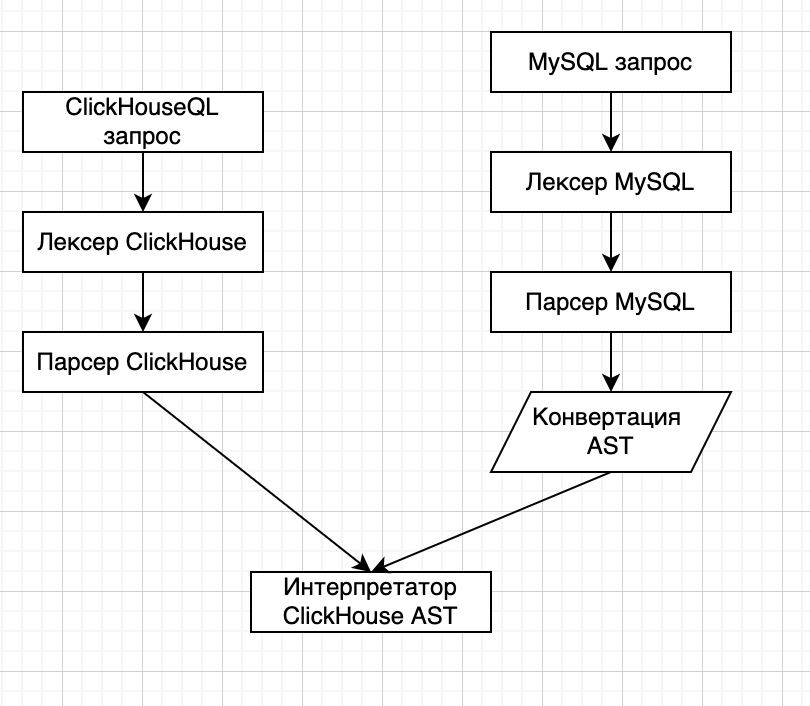
\includegraphics{images/general_conv_schema.jpg}
}
\caption{
\label{conv:general_pic} Общая схема конвертации MySQL запроса в диалект ClickHouse
}
\end{center}
\end{figure}

Ниже будут приведены фрагменты кода описывающие архитектуру конвертации MySQL AST в ClickHouse AST. Для большей лаконичности код упрощен и не содержит строк, не существенных для обещего понимания архитектуры. Полноценные версии используемых классов и реализации методов могут быть найдены в ветке \textbf{antlr-mysql-parser} \textit{форка} репозитория ClickHouse, созданного в ходе выполнения данной работы (TODO: сслыка на ветку в форке), а так же в соответсвующем \textit{Merge Request} в основной репозиторий ClickHouse \cite{merge_request}.

Для выбора диалекта языка запросов в ClickHouse была добавлена опция \textit{sql\_dialect}, которая может принимать два значения: \textit{mysql} либо \textit{clickhouse} (по умолчанию). Изменить диалект запросов в ClickHouse можно двумя способами:

\begin{enumerate}
    \item Посредством указания опции в файле конфигурации:\\ \mintinline{xml}{<profiles>}\\\mintinline{xml}{<default><sql_dialect>mysql</sql_dialect></default>}\\ \mintinline{xml}{</profiles>}
    \item Посредством запроса вида \mintinline{sql}{SET sql_dialect='mysql'}. Этим же способом можно переключиться обратно на диалект ClickHouse, если до этого был выбран диалект MySQL, т. к. реализована поддержка запросов \mintinline{sql}{SET} на диалекте MySQL (см. Раздел \ref{part:queries})
\end{enumerate}

Для того, чтобы успешно конвертировать ClickHouse AST в MySQL AST, необходимо извлечь нужную информацию из MySQL AST и придать ей структуру, соотвествующую структуре, порождаемой парсером ClickHouse при разборе запроса \textit{семантически аналогичного} данному. Ниже изложен метод, позволяющий эффективно осуществлять подобное преобразование в общем случае.

В фрагментах кода, приведенных ниже, за \mintinline{c++}{ MySQLPtr } обозначен умный указатель на MySQL AST, а за \mintinline{c++}{ CHPtr } - умный указатель на ClickHouse AST. Для поддержания общности будем называть тип AST, которое предстоит конвертировать \textit{исходным} (в данное работе - MySQL AST), а дерево, которое долнжо быть результатом преобразования \textit{целевым} (в данное работе - ClickHouse AST).

\subsection{Распознавание запроса} \label{conv:recognizer_}
Разбор запроса в ClickHouse устроен таким образом, что разным типам запросов соответсвуют ClickHouse AST с корнями разных типов (в отличае от MySQL AST, корнем которого всегда является вершина с типом \textit{query}). Исходя из этого, было принято решение сделать \textbf{распознание запроса} первым шагом конвертации.

Распознавание основано на объектах, классы которых реализуют интерфейс \mintinline{c++}{ IRecognizer } (см. Листинг \ref{conv:IRecognizer_cpp}), содержащий в себе метод \mintinline{c++}{ IRecognizer::Recognize }. Этот метод принимает на вход вершину MySQL AST и определяет, содержится ли в ее поддереве \textbf{корень} дерева, соответсвующего требуемому \textbf{типу запроса} (каждый наследник отвечает за специфический тип запроса). В случае успеха, метод возвращает вершину \textbf{дерева конвертации} (см. пункт \ref{conv_tree}), соответствующую корню нужного поддерева, в случае неудачи - \mintinline{c++}{ nullptr }.

\begin{code}
    \captionof{listing}{Архитектура распознавания запроса}
    \label{conv:IRecognizer_cpp}
    \begin{minted}[fontsize=\footnotesize, frame=single]{c++}
class IRecognizer
{
public:
    virtual ConvPtr Recognize(MySQLPtr node) const = 0;
    virtual ~IRecognizer() { }
};

class SelectQueryRecognizer : public IRecognizer
{
public:
    virtual ConvPtr Recognize(MySQLPtr node) const override;
};
    \end{minted}
\end{code}

Каждому типу запроса соответсвует своей наследник класса \mintinline{c++}{ IRecognizer }. Для того, чтобы применить все правила к каждой вершине MySQL AST используется \mintinline{c++}{ GenericRecognizer } (см. Листинг \ref{conv:GenericRecognizer}), содержащий в себе список доступных правил (поле \mintinline{c++}{ rules }) и осуществляющий распознание посредством поиска в грубину с поочередным применением всех правил к каждой рассматриваемой вершине. Результатом обобщенного распознания является результат первого правила, вернувшего не \mintinline{c++}{ nullptr }. 

\begin{code}
    \captionof{listing}{Структура GenericRecognizer}
    \label{conv:GenericRecognizer}
    \begin{minted}[fontsize=\footnotesize, frame=single]{c++}
class GenericRecognizer : public IRecognizer
{
public:
    virtual ConvPtr Recognize(MySQLPtr node) const override;

private:
    std::vector<IRecognizerPtr> rules = {
            std::make_shared<SetQueryRecognizer>(),
            std::make_shared<SelectQueryRecognizer>(),
            std::make_shared<UseCommandRecognizer>(),
            std::make_shared<ShowQueryRecognizer>(),
            std::make_shared<DescribeCommandRecognizer>()
        };
}
    \end{minted}
\end{code}

На момент написания работы, в ClickHouse внедрена поддержка распознания следующих типов запросов:
\begin{itemize}
    \item Запросы типа \mintinline{sql}{SELECT}
    \item Запросы типа \mintinline{sql}{SHOW}
    \item Запросы типа \mintinline{sql}{USE}
    \item Запросы типа \mintinline{sql}{SET}
    \item Запросы типа \mintinline{sql}{DESCRIBE}
\end{itemize}

Запросы, не соответсвующие типам, указанным выше, не подлежат конвертации. При попытке исполнить неподдерживаемые запросы будет возвращена ошибка. Остальные запросы будут однозначно соответсвовать поддерживаемым правилам, и будут конвертированы. Реузльтатом конвертации может быть либо ClickHouse AST, семантически аналогичное исходному MySQL AST, либо ошибка указывающая на то, что данный запрос корректен, но несовместим с ClickHouse, несмотря на то, что его тип поддерживается.

В дальнейшем планируется расширять типы поддерживаемых запросов на диалекте MySQL, а так же уменьшать число ошибок конвертации поддерживаемых запросов путем добавления в ClickHouse недостающей функциональности. 

\subsection{Деревья конвертации} \label{conv_tree}
Выше было упомянуто, что каждое правило распознавания возвращает указатель на \textbf{дерево конвертации} в случае успеха. Дерево конвертации - предложенная в рамках данной работы концепция преобразования исходного AST в целевое путем создания древовидной сущности, структура которой зависит от данных, содержащихся в исходном AST и требуемой формы целевого AST одновременно. 

Принцип работы дерева конвертации состоит в двух последовательных шагах: извлечение деревом конвертации инфорации из исходного AST и порождение деревом конвертации целевого AST. Дерево конвертации конструируется от некоторой вершины исходного AST, которая в дальнейшем будет именоваться источником данных (\textit{source node}). В процессе извлечения данных дерево конвертации может исполнить 3 типа действий:

\begin{enumerate}
    \item Сохранить в свои поля любые данные, содержащиеся в поддереве собственного источника данных, в подходящем формате
    \item Создать дочернее дерево конвертации, взяв за источник данных веришну, лежащую в поддереве собственного источника данных, после чего инициировать у него процесс извлечения данных, а затем записать его (но не данные им извлеченные) в свое поле. 
    \item Вернуть ошибку, если в источнике данных присутсвует информация, которую дерево конвертации не ожидает встретить или не может обработать
\end{enumerate}

На втором шаге (порождение целевого AST), дерево конвертации возвращает \textbf{ровно одну} вершину целевого AST (возможно, с потомками). Для этого дерево конвертации может исполнить 4 типа действий:

\begin{enumerate}
    \item Создать вершину целевого AST используя собственные поля, соответсвующие извлеченным данным (полученным путем действия типа 1 на шаге 1)
    \item Инициировать процесс порождения вершины целевого AST у одной из собственных \textbf{дочерних} вершин конвертации (полученных путем действия типа 2 на шаге 1)
    \item Образовать связь между любыми двумя вершинами целевого AST, полученными действиями 1 и 2
    \item Назначить одну из полученных вершин результатом (после создания необходимых связей) и завершить работу
\end{enumerate}

Структура дерева конвертации и его действия должны удовлетворять следующим требованиям
\begin{enumerate}
    \item Если процесс извлечения данных завершился ошибкой, порождение целевого AST не инициируется
    \item В процессе порождения целевого AST запрещается обращатся к исходному AST, а так же изменять структуру и поля дерева конвертации (включая дочерние деревья конвертации)
    \item Дерево конвертации не должно извлекать данные из поддеревьев, соответсвующих источникам данных его дочерних деревьев конвертации
\end{enumerate}

Предложенный метод обладает следующими важными положительными свойствами:
\begin{enumerate}
    \item Процесс порождения целевого дерева не зависит от структуры исходного дерева и деталей алгоритма извлечения данных (по построению алгоритма)
    \item Процесс порождения целевого дерева не может завершиться ошибкой и его результат всегда корректен (причиной ошибки может быть только неподдерживаемая структура исходного дерева, что определяется на шаге 1)
    \item После извлечения данных, дерево конвертации может породить произвольное количество идентичных целевых деревьев (следует из того, что в процессе порождения не меняется ни исходное AST, ни дерево конвертации)
\end{enumerate}

\subsection{Применение деревьев конвертации в ClickHouse}
Предложенная концепция дерева конвертации была реализована в ClickHouse с целью конвертировать MySQL AST в ClickHouse AST. Вершины дерева реализуют интерфейс \mintinline{c++}{ IConversionTree }, включающий в себя методы \mintinline{c++}{ IConversionTree::setup } (реализует извлечение данных из исходного AST) и \mintinline{c++}{ IConversionTree::convert } (реализует порождение целевого AST), а так же поле \mintinline{c++}{ IConversionTree::_source } - источник данных (см. Листинг \ref{conv:IConversionTree_cpp}).

\begin{code}
    \captionof{listing}{Интерфейс дерева конвертации}
    \label{conv:IConversionTree_cpp}
    \begin{minted}[fontsize=\footnotesize, frame=single]{c++}
class IConversionTree
{
public:
    IConversionTree(MySQLPtr source, const String & rule_name = "");
    virtual bool setup(String & error) = 0;
    virtual void convert(CHPtr & ch_tree) const = 0;
    virtual ~IConversionTree() { }

protected:
    MySQLPtr getSourceNode() const { return _source; }

private:
    MySQLPtr _source; // source node
};

using ConvPtr = std::shared_ptr<IConversionTree>;
    \end{minted}
\end{code}

На момент написания работы были реализованы следующие типы вершин конвертации:
\begin{enumerate}
    \item Деревья конвертации выражений \begin{enumerate}
        \item ExprGenericLiteralCT - конвертирует литералы (число, строка, TRUE, FALSE, NULL, и т. д.)
        \item ExprIdentifierCT - конвертирует индентификаторы (имена столбцов, алисов и т. д.)
        \item ExprVariableCT - конвертирует переменные
        \item ExprSumCT - конвертирует агрегатные функции
        \item ExprSimpleCT - конвертирует выражения с унарным минусом и вызовы функций
        \item ExprBitCT - конвертирует арифметические операции
        \item ExprBoolStatementCT - конвертирует выражения которые могут быть простыми логическими высказываниями
        \item ExpressionCT - конвертирует выражения, которые могут быть сложными логическими высказываниями
    \end{enumerate}
    \item Деревья конвертации запроса \mintinline{sql}{ SELECT } \begin{enumerate}
        \item SelectItemsListCT - конвертирует список выбираемых элементов
        \item SelectOrderByCT - конвертирует клаузу \mintinline{sql}{ ORDER BY } 
        \item SelectLimitOffsetCT - конвертирует смещение в выражении \mintinline{sql}{ LIMIT } 
        \item SelectLimitLengthCT - конвертирует размер в выражении \mintinline{sql}{ LIMIT } 
        \item SelectTableCT - конвертирует идентификатор таблицы
        \item SelectFromCT - конвертирует клаузу \mintinline{sql}{ FROM } 
        \item SelectGroupByCT - конвертирует клаузу \mintinline{sql}{ GROUP BY} 
        \item SelectQueryExprCT - конвертирует запрос \mintinline{sql}{ SELECT }
        \item SelectQueryCT - вспомогательное дерево, нужное для совместимости с ClickHouse AST
    \end{enumerate}
    \item Деревья конвертации запроса \mintinline{sql}{ SHOW } \begin{enumerate}
        \item ShowColumnsCT - конертирует запрос вида \mintinline{sql}{ SHOW COLUMNS } 
        \item ShowTablesCT - конвертирует запрос вида \mintinline{sql}{ SHOW TABLES; } 
        \item ShowQueryCT - конвертирует запросы \mintinline{sql}{ SHOW } в общем виде 
    \end{enumerate}
    \item Прочие деревья конвертации \begin{enumerate}
        \item SetQueryCT - конвертирует запросы \mintinline{sql}{ SET } 
        \item UseCommandCT - конвертирует запрос \mintinline{sql}{ USE databasee; } 
        \item DescribeCommandCT - конвертирует запрос \mintinline{sql}{ DESCRIBE }
    \end{enumerate}
\end{enumerate}

Точка входа, запускающая процесс распознания запроса, с последующим созданием и использованием дерева конвертации выглядит следующим образом (см. Листинг \ref{conv:EntryPoint}):

\begin{code}
    \captionof{listing}{Точка входа в процесс конвертации}
    \label{conv:EntryPoint}
    \begin{minted}[fontsize=\footnotesize, frame=single]{c++}
bool Converter::toClickHouseAST(const String & query, 
                CHPtr & ch_tree, String & error) const
{
    MySQLPtr root = nullptr;
    MySQLTree::FromQuery(query, root, internal_error);

    // invalid MySQL query error handling

    GenericRecognizer recognizer;
    
    auto result = recognizer.Recognize(root);
    result->setup(internal_error);

    // failed conversion error handling

    result->convert(ch_tree);

    return true;
}
    \end{minted}
\end{code}

\begin{figure}[ht]
\begin{center}
\scalebox{0.25}{
    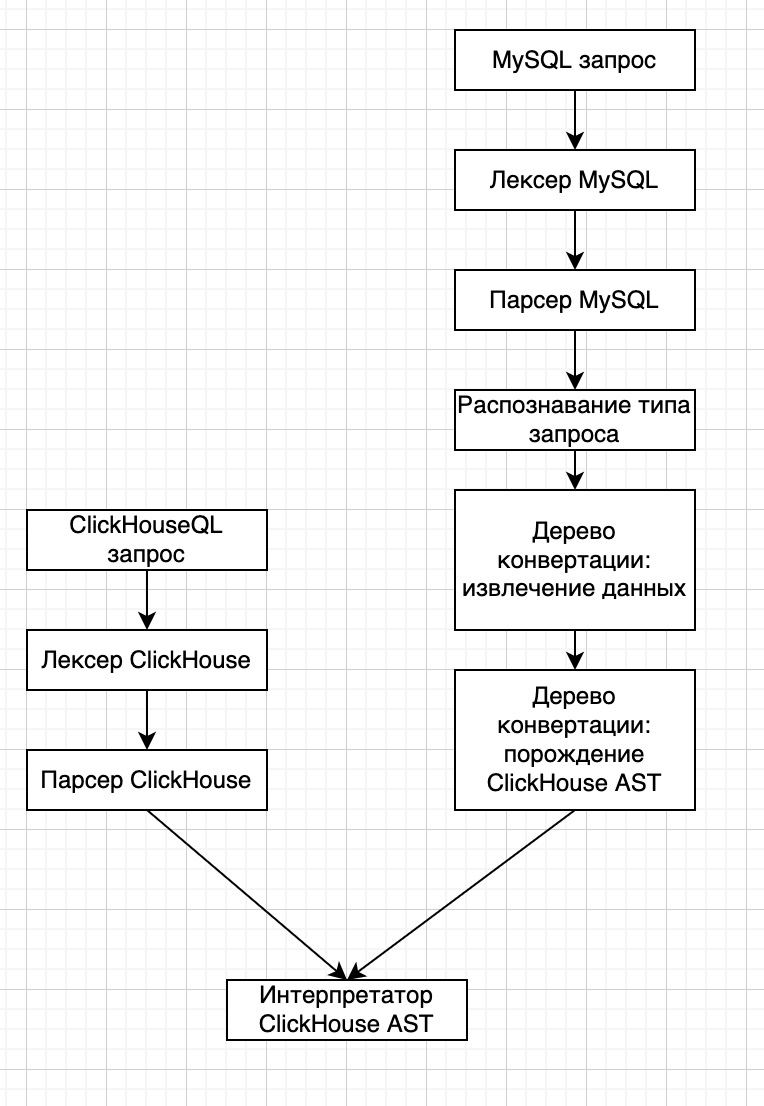
\includegraphics{images/spec_conv_schema.jpg}
}
\caption{
\label{conv:spec_pic} Схема конвертации MySQL AST в ClickHouse AST
}
\end{center}
\end{figure}


С учетом описанного выше, схему архитектуры процесса конвертации запроса на диалекте MySQL в ClickHouse, изложенную в начале главы (см. Рис. \ref{conv:general_pic}), можно дополнить до следующего вида (см. Рис. \ref{conv:spec_pic}):

\subsection{Множество поддерживаемых запросов} \label{part:queries}
Алгоритм преобразования MySQL AST в ClickHouse AST, использующий метод деревьев конвертации позволил поддержать следующее подножество корректных запросов на диалекте MySQL:
\begin{itemize}
    \item Запрос \mintinline{sql}{ USE databasee; }
    \item Запрос \mintinline{sql}{ DESCRIBE table; }
    \item Запрос вида \mintinline{sql}{ SET key1=val1, key2=val2, ... }, где key - переменная, а val - литерал
    \item Запросы вида \mintinline{sql}{ SHOW TABLES } и \mintinline{sql}{ SHOW COLUMNS FROM }
    \item Запросы \mintinline{sql}{ SELECT }:
    \begin{itemize}
        \item Не содержащие \mintinline{sql}{ JOIN } и \mintinline{sql}{ UNION }
        \item Поддерживающие выражения в списке выбираемых элементов
        \item Поддерживающие \mintinline{sql}{ WHERE }, \mintinline{sql}{ ORDER BY }, \mintinline{sql}{ GROUP BY }, \mintinline{sql}{ HAVING } и \mintinline{sql}{ LIMIT }
        \item Поддерживающие агрегатные функции 
        \begin{itemize}
            \item \mintinline{sql}{ sum }
            \item \mintinline{sql}{ count }
            \item \mintinline{sql}{ min }
            \item \mintinline{sql}{ max }
            \item \mintinline{sql}{ avg }
            \item \mintinline{sql}{ stddev_pop}
            \item \mintinline{sql}{ stddev_samp }
            \item \mintinline{sql}{ var_pop }
            \item \mintinline{sql}{ var_samp }
        \end{itemize}
        \item Поддерживающие подзапросы вида \\ \mintinline{sql}{ SELECT ... FROM (SELECT ...) ...; }
    \end{itemize}
\end{itemize}

Поддерживаемый синтаксис не является исчерпывающим, однако, предложенный метод конвертации позволяет легко итеративно расширять подмножество поддерживаемых запросов.
